\chapter{Ausgangssituation}
\label{chap:three}
Im folgenden Kapitel wird die wissenschaftliche Spezialbibliothek des \textit{Max-Planck-Institutes für empirische Ästhetik} porträtiert,
um die Ausgangslage für die vorliegende Arbeit zu umreißen.
Anschließend werden die bibliothekarischen Informationsdienstleistungen der Bibliothek skizziert und der Frage nachgegangen, 
welche statistischen Daten bisher aggregiert und ausgewertet werden. Diese Daten stellen die Basis für die spätere Konzeption und Entwicklung des datengetriebenen Unterstützungssystems dar.
\footnote{Da für die Auswertung keine personenbezogenen Daten wie Nutzer:innendaten analysiert werden, wird das wichtige Thema des Datenschutzes sowie
die Pseudonymisierung beziehungsweise Anonymisierung personenbezogener Daten hier nicht erörtert. Neben den personenbezogenen Daten gibt es noch interne betriebliche Daten. Diese sind in der vorliegenden Arbeit entweder 
randomisiert oder (in Abbildungen) unkenntlich gemacht worden. } 

\section{Bibliothek}
\label{chap:three_one}
\subsection{Allgemeines}
%Wann wurde die Bibliothek gegründet?\\
Die Spezialbibliothek wurde im Zuge der Gründung des \textit{\acrshort{MPI EA}}
in Frankfurt im Jahr 2013 gegründet. Die Aufgabe des Institutes ist die interdisziplinäre Erforschung 
empirischer Fragestellungen der Ästhetik. Das Institut besteht derzeit aus den drei Abteilungen \textit{Sprache und Literatur}, 
\textit{Musik} und \textit{Neurowissenschaften} sowie einigen Forschungsgruppen. %Ungefähr 150 Mitarbeiter:innen 
%arbeiten in dem Institut. 



% Warum wurde die Bibliothek gegründet?
%Welche Aufgaben hat die Bibliothek?
%Welche Servicedienstleistungen bietet die Bibliothek an?
Die Bibliothek ist eine Serviceeinrichtung des Institutes und dient mit ihren Informationsdienstleistungen 
der Forschung.
Zentral ist dabei die Informationsversorgung der Forschenden. Die benötigten Informationen sind Bücher, 
Zeitschriften, Zeitschriftenartikel sowohl in gedruckter als auch in elektronischer Form.
%Seit der Institutsgründung wird neben des nutzungsorientierten Bestandaufbaus ebenfalls eine planmäßige 
%Bestandsentwicklung betrieben. Das Erwerbungsprofil der Bibliothek leitet sich aus dem Forschungsauftrag des Institutes 
%ab und umfasst dementsprechend die Erwerbung von Informationsressourcen, die sich den theoretischen und 
%empirischen Fragestellungen der Ästhetik widmen.
%Wie groß ist der Bibliotheksbestand? 
Der Bibliotheksbestand ist somit hybrid. Er besteht sowohl aus gedruckten als auch aus Online-Medien sowie 
audiovisuellen Materialien. An Bestand umfasst die Bibliothek über 11.000 Bücher, circa 30 laufende Zeitschriften, 
knapp 200 audiovisuelle Medien sowie Online-Datenbanken und Online-Zeitschriften.\footnote{Stand: Dezember 2020}

\subsection{Organisatorische Einbettung}
%Wie sieht der größere Organisationsrahmen der Bibliothek aus?\\
Um alle Informationsbedarfe der Forscher:innen zu befriedigen, wird die Bibliothek in ihren Aufgaben von der
\textit{\acrlong{mpdl}} unterstützt. Deren Portfolio umfasst vorrangig die zentrale 
Lizenzierung von relevanten elektronischen Informationsressourcen, die Bereitstellung von Softwarelösungen, 
das Betreiben des Publikationsrepositoriums \textit{\acrshort{PuRe.MPG}} der \textit{\acrlong{MPG}} sowie
das Vorantreiben von Open-Access-Initiativen. 

Darüber hinaus ist die Spezialbibliothek Teil des \textit{\acrshort{hebis}-Verbundes}. 
Seit Ende 2014 finden die Geschäftsprozesse der Katalogisierung und der Erwerbung im \textit{\acrfull{CBS}} und 
im Lokalsystem \textit{\acrfull{LBS}} vom \textit{\acrshort{OCLC}} in einem integrierten Geschäftsgang statt. Im \textit{\acrfull{OPAC}} befinden sich Bücher, ausgewählte E-Books 
und Zeitschriften (Print und Online) der Institutsbibliothek. Lokal lizenzierte Datenbanken finden sich dagegen
nicht im Katalog. Das \textit{\acrshort{LBS}} wird gehostet und betreut 
vom Lokalsystem-Team Frankfurt. Als Service-Leistungen werden der Bibliothek besondere Funktionalitäten 
für das \textit{\acrlong{CBS}} und Statistiken aus dem \textit{\acrshort{LBS}} bereitgestellt.


\subsection{Informationsdienstleistungen}
Das Bibliotheks-Team des \textit{\acrshort{MPI EA}} ist verantwortlich für den Ablauf und die Organisation der bibliothekarischen 
Informationsdienstleistungen. Eine Übersicht der Informationsdienstleistungen,
aufgeschlüsselt nach den Basisfunktionen einer Bibliothek \cite[S. 204 f.]{rosch_bibliotheken_2019}, zeigt \autoref{tab:Informationsdienstleistungen}. 
Die zentralen Informationsdienstleistungen der Spezialbibliothek bestehen aus der Sammeltätigkeit und dem Benutzungsservice.
Seit der Institutsgründung wird neben dem nutzer:innengesteuerten Bestandsaufbau ebenfalls eine planmäßige 
Bestandsentwicklung betrieben. Das Erwerbungsprofil der Bibliothek leitet sich aus dem Forschungsauftrag des Institutes 
ab und umfasst dementsprechend die Erwerbung von Informationsressourcen, die sich den theoretischen und 
empirischen Fragestellungen der Ästhetik widmen.


Die Dienstleistungsbereiche der Benutzung sind zuständig für die Organisation der Fern- und Ortsleihe 
von Informationsressourcen, die nicht in das Erwerbungsprofil der Spezialbibliothek fallen. Ferner sind diese 
für die Informationsbeschaffung sowohl über Dokumentenlieferdienste als auch für die Akquise einzelner Zeitschriftenaufsätze zuständig.

\begingroup
\setlength{\tabcolsep}{12pt} % Default value: 6pt
\renewcommand{\arraystretch}{1.5} 
\begin{table}[h]
    \centering
    \begin{adjustbox}{max width=\textwidth}
    \begin{tabular}{p{0.4\textwidth}p{0.9\textwidth}}
       \toprule
       Basisfunktion                            & Beschreibung\\
       \midrule
        Benutzung                               &Ausleihe, Lesesaalnutzung, Organisation der Lieferdienste (Fern- und Ortsleihe, Dokumentenlieferdienste)\\
        Management techn. Infrastruktur         &\textit{\acrshort{PuRe.MPG}}, Medien-Datenbank\\
        Ordnen                                  &Aufstellungssystematik \textit{\acrshort{RVK}}\\
        %Sammeln bes. Materialien                &Stimulus wie Musikstücke, Bilder, Textlizenzen, Zeitschriftenartikel\\
        Sammeln und Erschließen                 &geplanter Bestandsaufbau, Integrierter Geschäftsgang Medienerwerbung und Medienerschließung, besondere Materialien\\
        Vermitteln                              &Literaturrecherche, Nutzung elektronischer Ressourcen, Urheberrecht und Publikationsberatung\\
   
       \bottomrule
    \end{tabular}
    \end{adjustbox}
    \caption
    \end{table}
\endgroup

Der Bestand wird nach den \textit{\acrshort{RVK}}-Fachsystematiken inhaltlich erschlossen und an diese angelehnt geordnet aufgestellt.
Weitere Informationsdienstleistungen der Bibliothek sind die Betreuung des Publikationsrepositoriums \textit{\acrshort{PuRe.MPG}} des Institutes, spezielle Beratungsdienstleistungen 
zum Urheberrecht und zum Publishing sowie klassische Auskunfts- und Informationsdienste. Seit Beginn 2016 
geschieht die Ausleihe der Medien über ein Selbstverbuchungssystem.\\
%Nutzergruppen

\subsection{Evaluation der Informationsdienstleistungen}

Zu fast jeder Informationsdienstleistung der Spezialbibliothek werden quantitative Daten elektronisch erhoben. 
Die \autoref{tab:Statistische_Daten} zeigt Daten, die bereits jetzt in der ein oder anderen Form aggregiert und ausgewertet werden. 
Die Tabelle stellt nach den Evaluationstypen dar, in welcher Frequenz die Statistiken erfasst werden. Ferner bietet sie einen Überblick darüber, in welchem 
Dateiformat die Daten vorliegen, über die Quellen aus der die Daten stammen, und ob die Daten bereits ausgewertet und/oder visualisiert werden.\footnote{ Folgende
Abkürzungen werden in der Tabelle verwendet: E = Evaluationstyp, N = Nutzungsbezogen, S = Sammlungsbezogen, XLSX = Excel Spreadsheet XML, TSV = Tab-separated values, TXT = Plain-Text}


\begingroup
\setlength{\tabcolsep}{4pt} % Default value: 6pt
%\renewcommand{\arraystretch}{1.5}
%\resizebox{\textwidth}{!}{
\begin{table}[H]
    \centering
    \large
    \begin{adjustbox}{max width=\textwidth}
    \begin{tabular}{p{0.1\textwidth}p{0.2\textwidth}p{0.3\textwidth}p{0.2\textwidth}p{0.2\textwidth}p{0.2\textwidth}p{0.2\textwidth}p{0.15\textwidth}p{0.2\textwidth}}
    %\begin{tabular}{lllclllcc}
      %\begin{tabular}{p{3cm}p{5cm}p{1cm}p{1.5cm}p{2cm}p{4cm}}
       \toprule
       \textbf{E} &\textbf{Basisfunktion}               &\textbf{Daten}                                 &\textbf{Zeitraum} &\textbf{Frequenz}    &\textbf{Quelle}  &\textbf{Dateiformat}          &\textbf{Auswer-tung} & \textbf{Visualisierung}\\
       \midrule     
            N         &Benutzung                      & Ausleihzahlen Bibliotheksbestand              & 2016-             & unregelmäßig         & LBS          & Mail, XLSX              & nein  & -\\
            N         &Benutzung                      & Ausleihzahlen Lieferdienste                   & 2015-             & monatlich         & intern       & XLSX                      & ja    & teilweise, Li-niendiagramm\\ 
            N         &Benutzung                      & Besonders nachgefragte Medien (OPAC)          & 2017-             & monatlich         & LBS          & Mail, TXT                 & nein  & -\\ 
            N         &Sammeln                       &\acrshort{COP 5}-Statistiken elektr. Ressourcen& 2013-            & unbekannt                 & mpdl         & CSV, TSV, TXT             & nein  & -\\ 
            N         &Benutzung                      & Lesesaalnutzung                               & 2017-             & wöchentlich       & intern       & XLSX                      & nein  & -\\ 
            %Sammeln bes. Materialien        & Anzahl der Materialien                       & unregelmäßig      & unregelmäßig      & intern       & XLSX                      & nein  & -\\
            S         &Sammeln                       & Budget nach Kostenstellen                   & 2018-               & monatlich         & LBS          & Mail, TXT                 & ja    & -\\ 
            S         &Sammeln                       & Umsatz nach Lieferanten                     & 2018-               & monatlich         & LBS          & Mail, TXT                 & ja    & Balken- und Kreisdiagramm\\ 
            S         &Sammeln                       & Größe und Art des Bestandes                   & 2014-             & jährlich          & LBS, intern  & CSV                       & nein  & -\\ 
            S         &Sammeln                       & Neuerwerbungslisten                           & 2014-             & unregelmäßig         & LBS, intern  & TSV                       & nein  & -\\ 
            

        \bottomrule
    \end{tabular}
    \end{adjustbox}
    \caption
    \label{tab:Statistische_Daten}
    }
     \end{table}

\endgroup


Intern erfasst die Bibliothek monatlich die Daten der Ausleihe über die Lieferdienste. Unterschieden 
wird in der Erfassung nach Medientypen, nach Ausleihort und Ausleihart. Zudem werden wöchentlich 
Statistiken zur Nutzungshäufigkeit des Lesesaals geführt. Jährlich wird für die Buchhaltung die Bestandsgröße ermittelt.

Die Neuerwerbungsdaten können von der Bibliothek selbständig aus dem \textit{\acrshort{CBS}} abgezogen werden. Diese werden aus
dem bibliotheksinternen PICA3-Format\footnote{ Zum Aufbau des Datenformats und der Titel- und Lokaldaten im \textit{\acrlong{CBS}} \cite[vgl.][4]{hebis_datenstruktur_2017}.}
in einer TSV-Datei gespeichert. Folgende \autoref{fig:Bestandsdaten}\footnote{Die Spaltenüberschriften wurden fett hervorgehoben
und die Spalten sind zum Teil ineinander verschoben. Für die Verantwortliche Person und die \textit{\acrshort{RVK}-Fachsystematiken}
werden auch die Identifikationsnummern des \textit{\acrlong{CBS}s} mitgeliefert.} zeigt in tabellarischer Darstellung
die Daten einer solchen Neuerwerbungsdatei.
Die Neuerwerbungsdaten enthalten neben internen Identifikationsnummern (ppn und epn) unter anderem die Titeldaten für die bibliographische Beschreibung der Ressourcen wie
Materialart (500), Erscheinungsjahr (1100), Verantwortliche Personen (3000 und 3010), Titel (4000) oder auch \textit{\acrshort{RVK}}-Fachsystematiken (5090).
Außerdem enthalten sie Lokaldaten wie die Signaturen (Signatur) für die Beschreibung der vorhandenen Exemplare in der Bibliothek.

\begin{figure}[H]
    \centering
        \includegraphics[width=14.5cm, height=5cm]{bestandsdaten}
        %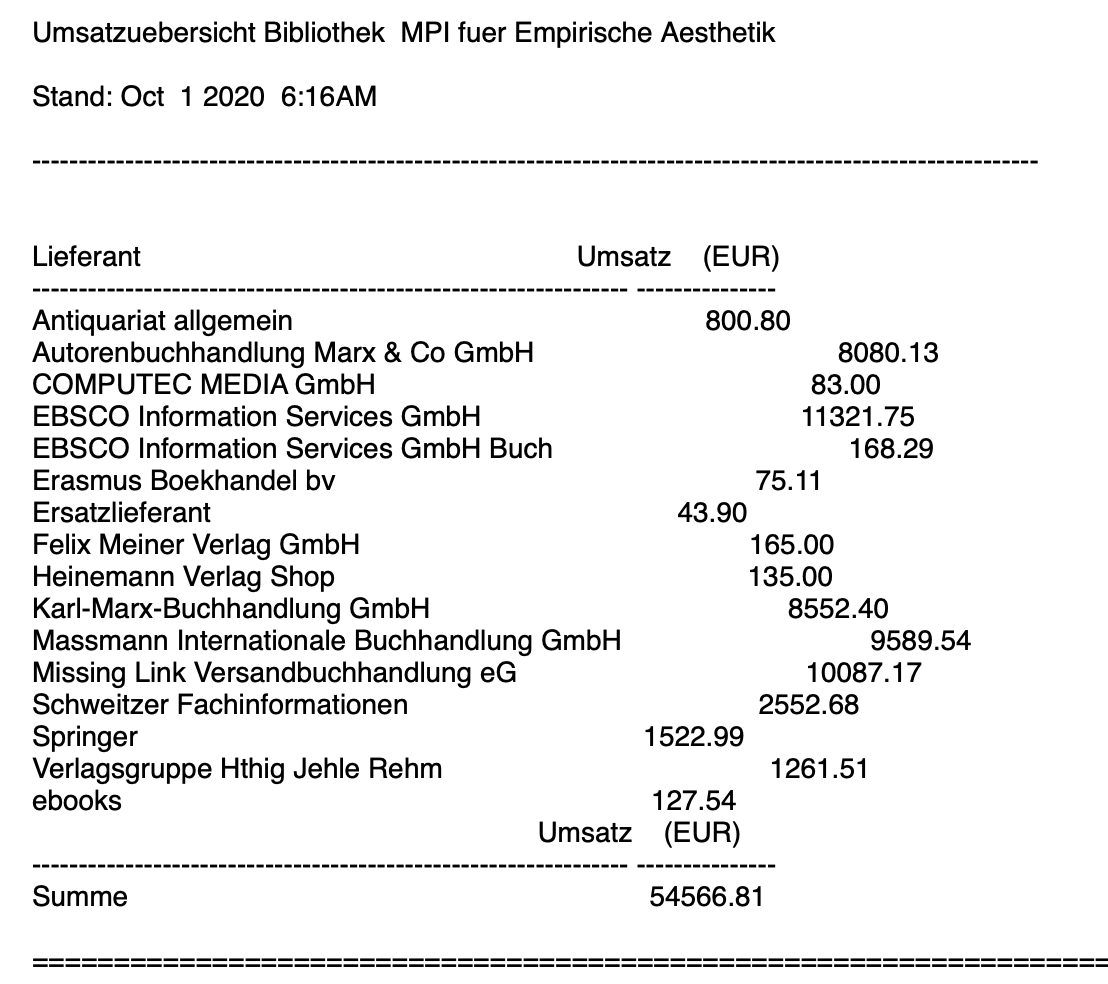
\includegraphics[width=6.5cm, height=6cm]{umsatzuebersicht}
        \caption{Neuerwerbungsdaten TSV-Datei}
        \label{fig:Bestandsdaten}
\end{figure}


Die Ausleihzahlen des Bibliotheksbestandes werden bei Bedarf durch das Lokalsystem-Team ermittelt und an die Bibliothek übermittelt. 
Diese liegen kumulativ nach Ausleihanzahl des einzelnen Titels oder nach Jahr und der Identifikationsnummer des Titeldatensatzes im 
\textit{\acrshort{CBS}} vor. Ebenfalls stehen die Ausleihzahlen als Rohdaten, in denen jede Titelausleihe über die Jahre aufgeführt wird, zur Verfügung.
Eine Auswertung dieser Ausleihzahlen findet bisher noch nicht statt. Die \autoref{fig:Titelausleihen} zeigt einen Auszug aus den Rohdaten der Ausleihzahlen mit 
unter anderem den PICA-Indentifikationsnummern (ppn und epn), der Exemplaranzahl (occurence), der Signatur (shelfmark), dem Kurztitel (shorttitle),
dem Jahr sowie den Ausleihinformationen (cum\_loans, cum\_request, cum\_reservations).


\begin{figure}[H]
    \centering
        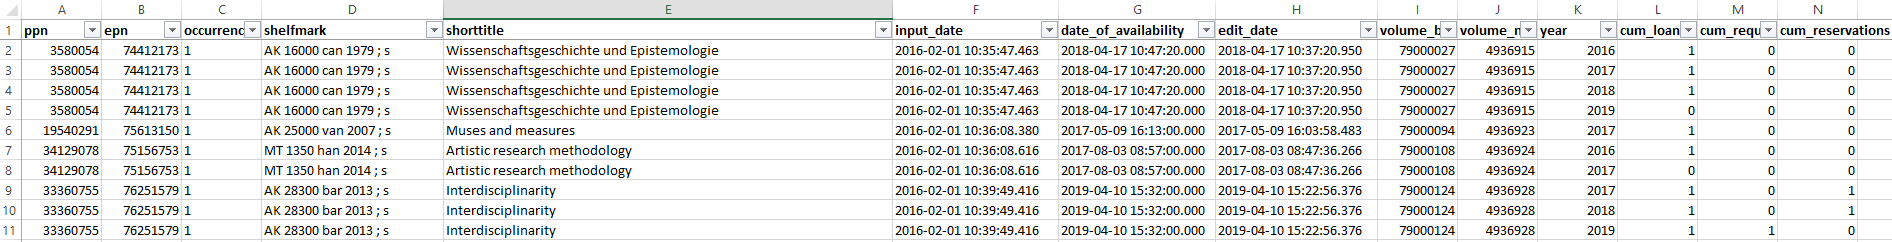
\includegraphics[width=14cm, height=6cm]{rohdaten_ausleihzahlen}
        %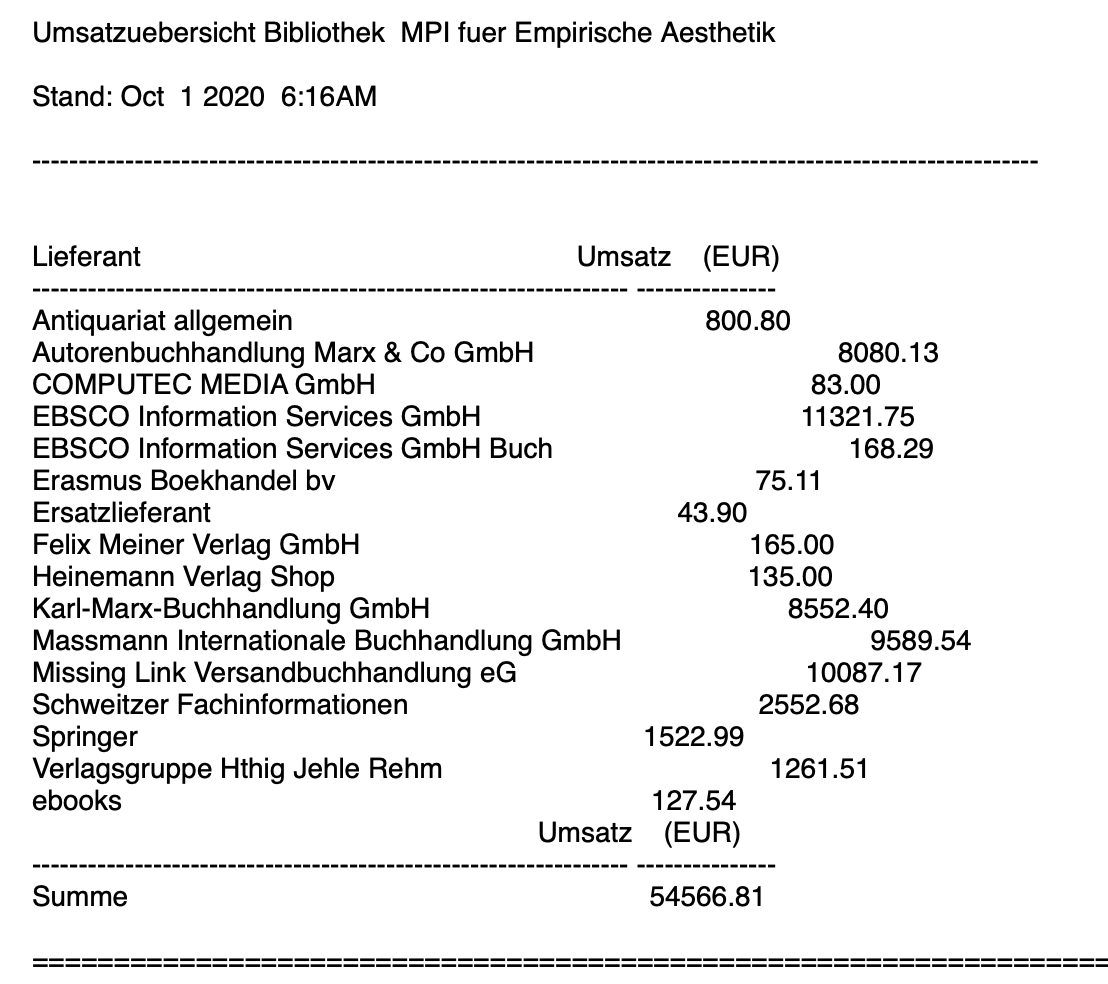
\includegraphics[width=6.5cm, height=6cm]{umsatzuebersicht}
        \caption{Rohdaten Ausleihzahlen XLSX-Datei}
        \label{fig:Titelausleihen}
\end{figure}


Monatlich bekommt die Bibliothek kumulative Umsatz- und Budgetübersichten der Lieferanten und der Kostenstellen zugeschickt.
Die Umsatzübersicht summiert die monatlichen Ausgaben nach Lieferanten bezogen auf das Kalenderjahr. Kriterium ist hierbei das Erfassungsdatum der Rechnung im \textit{\acrshort{LBS}}. 
Die Budgetübersicht gibt den monatlichen Stand der Budgets (Bindungen und Ausgaben) der einzelnen Kostenstellen zwischen den systeminternen Jahresübergängen an.\footnote{ Der
interne Jahresübergang variiert und der Zeitpunkt wird von der Bibliothek mit dem Lokalsystem-Team festgelegt. Der Jahresübergang geschieht meistens in den ersten beiden Januarwochen des Jahres.}
Die Kostenstellen bilden die einzelnen Abteilungen und zum Teil die Forschungsgruppen des Institutes ab.
Bearbeitet werden von der Bibliothek nur die Umsatzübersichten der Lieferanten, um die Umsatzverteilung nach Lieferanten zu steuern.
Die \autoref{fig:budget- und umsatzuebersicht} zeigt ein Beispiel\footnote{ Die Zahlen wurden zurückgesetzt und die Namen der Lieferanten sowie der Kostenstellen pseudonymisiert.}
vom November 2020 für die Umsatz- und Budgetübersichten des Monats Oktober 2020, die vom Lokalsystem-Team als Email zur Verfügung gestellt werden.


\begin{figure}[h]
    \centering
        %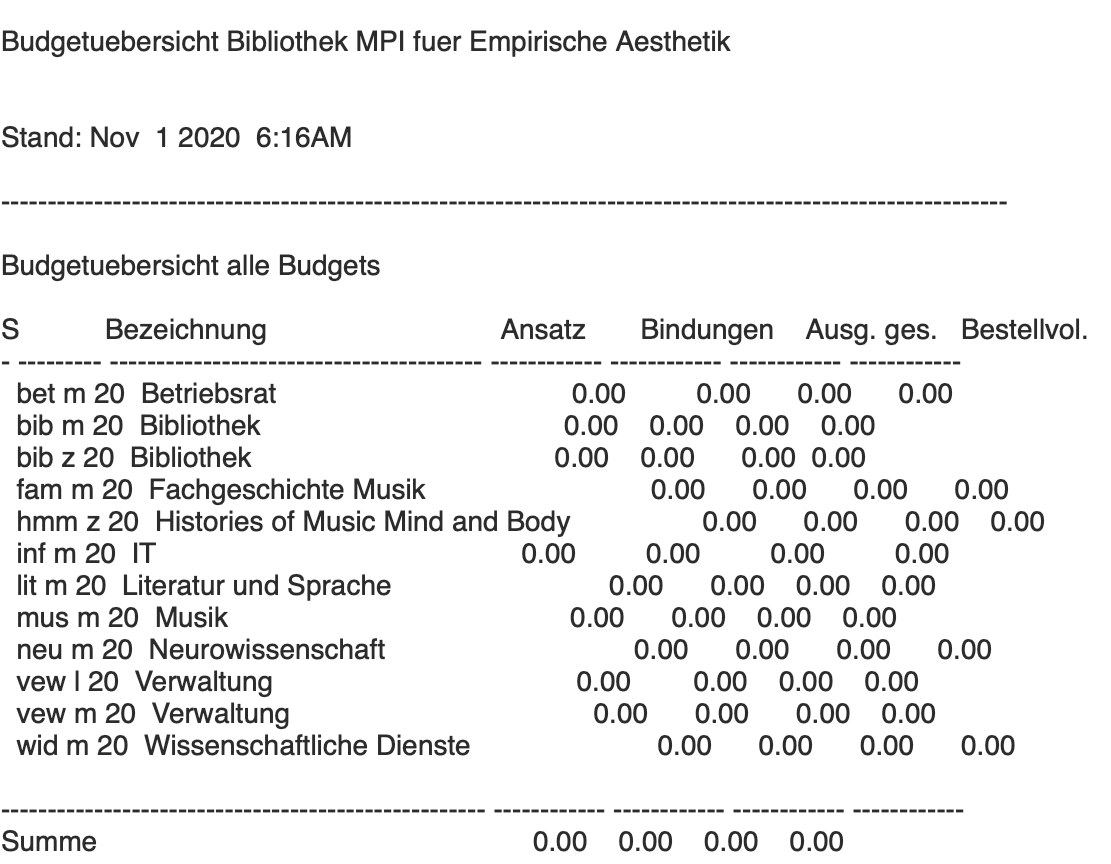
\includegraphics[width=6.5cm, height=9.0cm]{budget_uebersicht_mtl}
        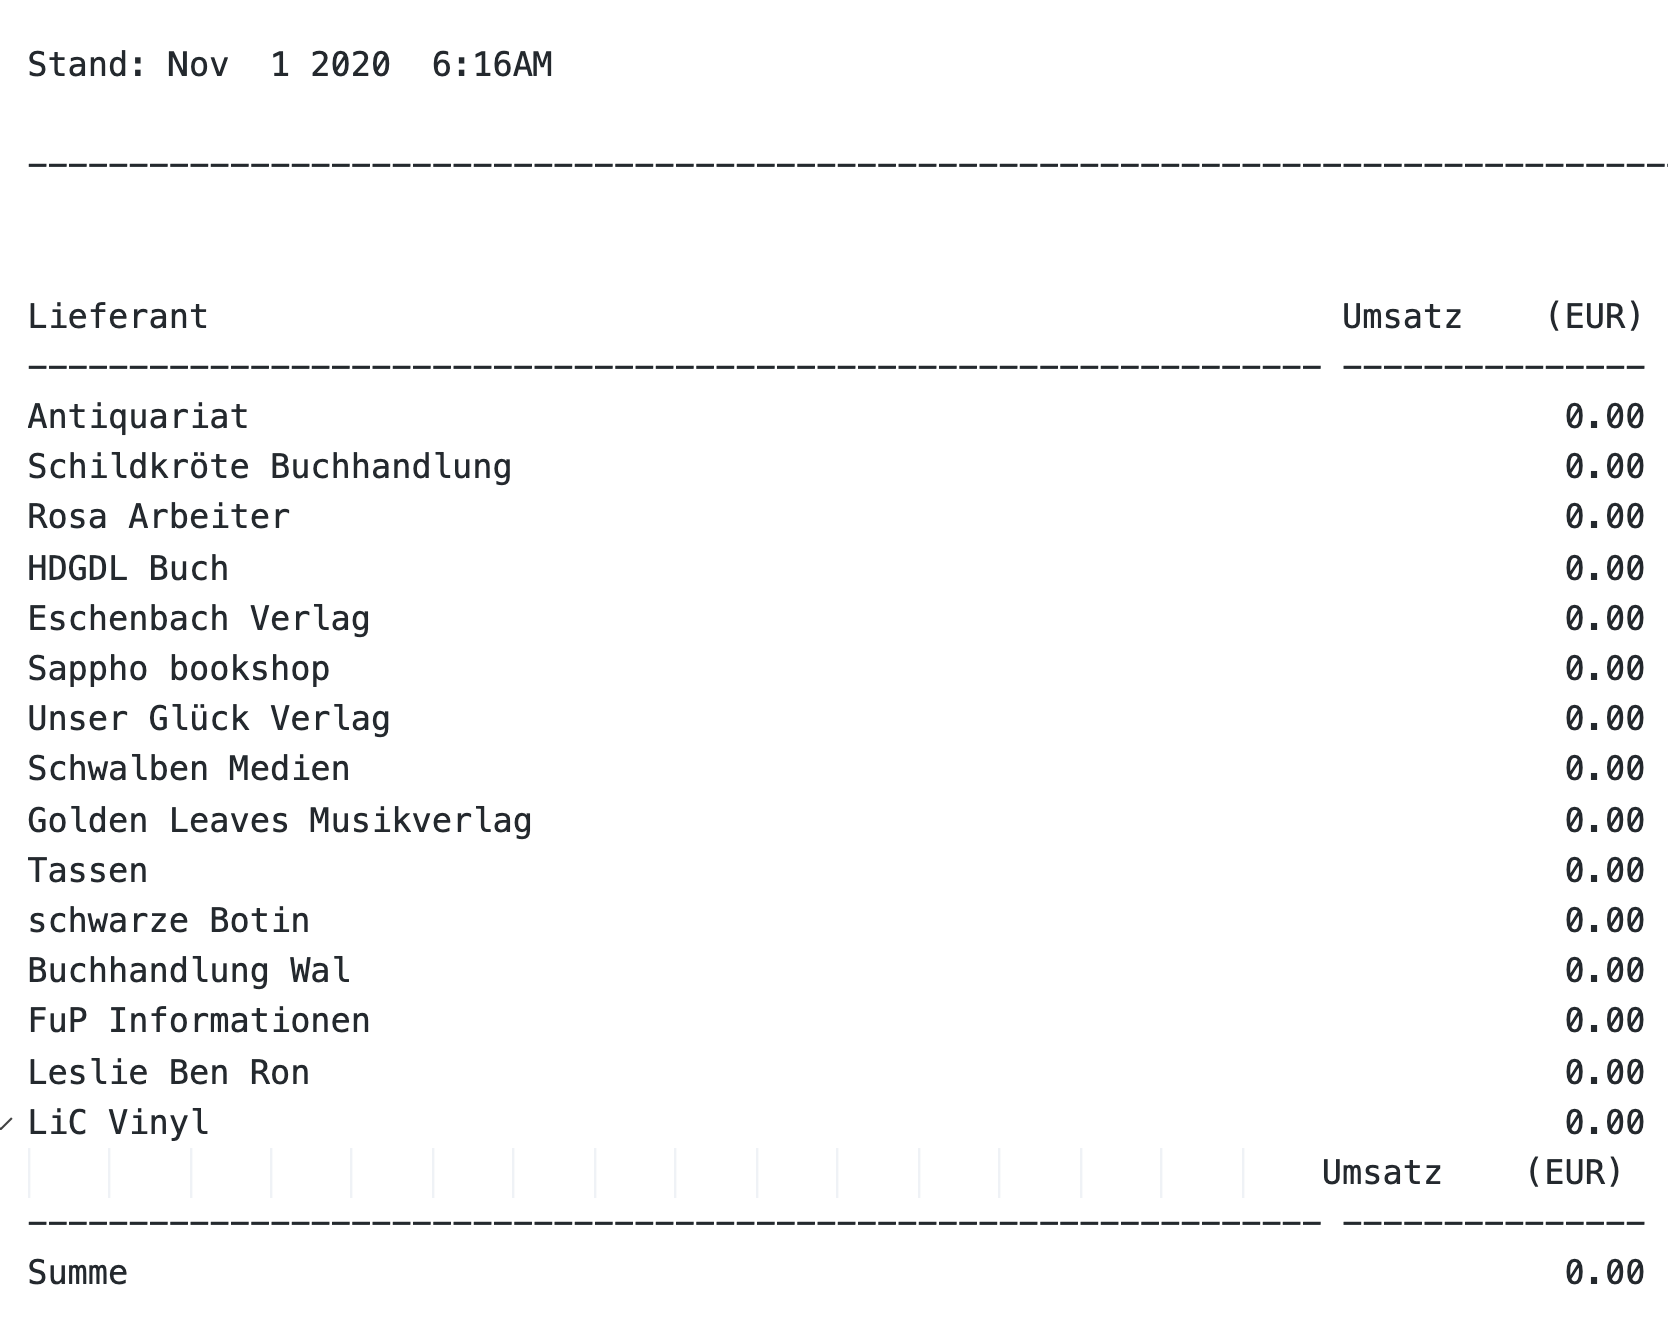
\includegraphics[width=6.0cm, height=8.0cm]{umsatzuebersicht_mtl}
        \includegraphics[width=7.5cm, height=8.0cm]{mtl_busget_uebers}
        \caption{Monatliche Umsatz- und Budgetübersicht}
        \label{fig:budget- und umsatzuebersicht}
\end{figure}

Die Ausgaben für die lokal lizenzierten Datenbanken fehlen in der Aufstellung der Ausgaben und werden in einer Tabelle extra geführt.

Die \textit{\acrfull{COP 5}} der Verlage werden dem Institut auf einen internen Portal der \textit{\acrshort{mpdl}} zur Verfügung gestellt.
Diese Statistiken verzeichnen den Zugriff innerhalb der IP-Adressbereiche des Institutes auf die elektronische Ressourcen, 
die konsortial durch die \acrshort{MPG} lizenziert wurden. Darunter fallen E-Books der Verlage 
\textit{Springer}, \textit{Wiley} oder \textit{De Gruyter}. Bisher werden diese von der Bibliothek weder gesichtet noch ausgewertet.
% Von seitens der Bibliothek wurden diese Statistiken leider noch nicht angefasst.

Eine proaktive und systematische Auswertung der Entwicklung der Bestandsgröße, der Ausleihzahlen und der \textit{\acrshort{COP 5}}-Statistiken findet nicht
oder nur unzureichend statt. 
% Auch wird das Potential hinsichtlich der Umsatz- und Budgetplanung wie in \autoref{chap:two_one} beschrieben nicht ausgeschöpft.

%\section{Zusammenfassung}

